\begin{frame}{Experiment 1}
\setbeamercovered{invisible}
\fontsize{12pt}{15}\selectfont
\only<1>{
\begin{center}
    {\Large\textbf{Experimental design:}}\\
    \vspace{1cm}
    {\Large 1$^{st}$ Task \hspace{2cm} \textbf{2$^{nd}$ Task}}
\end{center}}
\pause
\only<2>{
{\large\textbf{2$^{nd}$ Task:}}\\
{\large\textbf{To capture the overlap of syntactic and tool-use networks}}
\begin{itemize}
\item Same participants were asked to use a pair of \textbf{pliers} or their free right hand
\item Had to \textbf{move a peg} from one side of a board to the other
\item Recorded brain activity and isolated portion about \textbf{tool movement planning}
\end{itemize}}
\pause
\only<3>{\begin{figure}
    \centering
    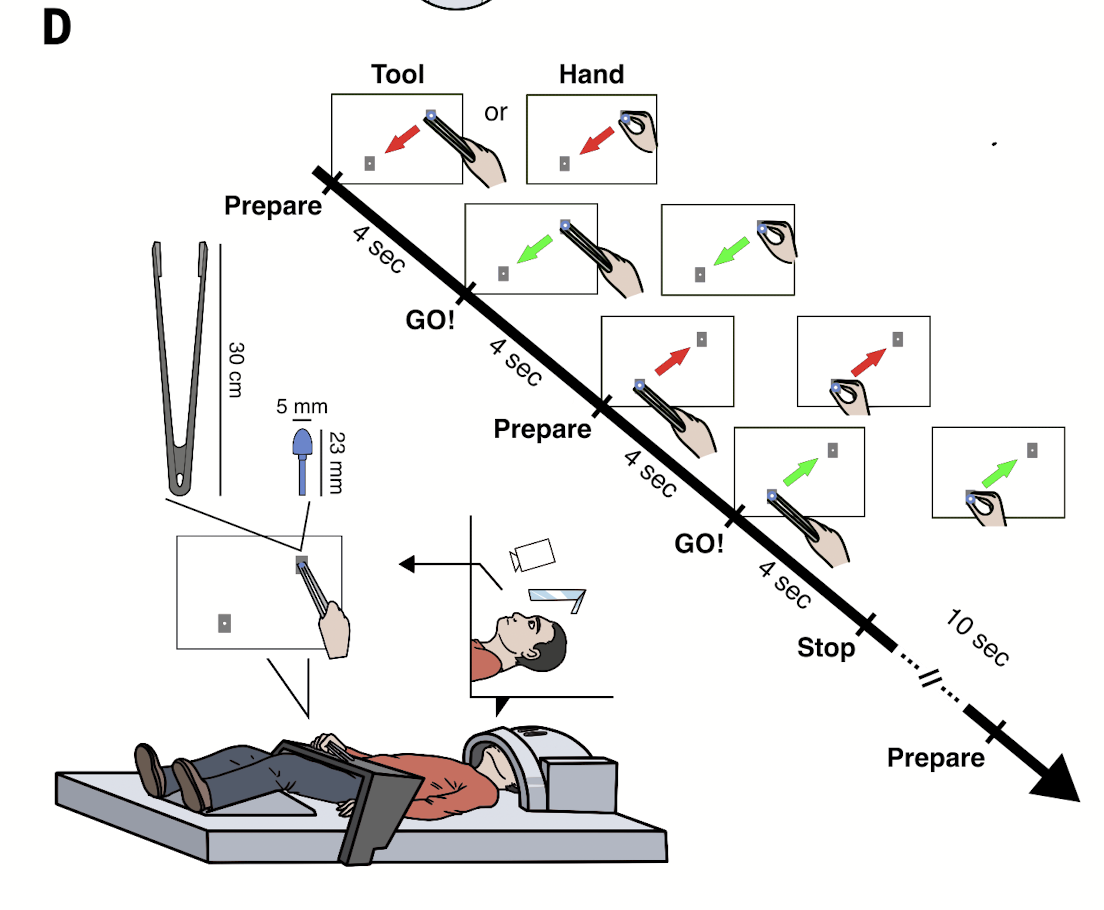
\includegraphics[width=8cm]{images/paper_pics/fig1D.png}
    %\caption*{}
    \label{fig:label3}
\end{figure}}
\pause
\only<4>{{\large\textbf{Results:}}
\begin{itemize}
    \item \textbf{Tool-use planning} found activation in parietal and prefrontal areas, and \textbf{BG} (both caudate nuclei, interbal globus pallidus, putamen). 
    \item Also ventral premotor cortex (within left IFG), though more posterior than findings for syntactic network.
\end{itemize}}

\end{frame}